\documentclass[11pt]{article}

% --- Nature Human Behaviour: Article format ---
% Main text: up to 5,000 words (excluding abstract, Methods, references,
%            figure legends)
% Abstract: <=150 words, unreferenced
% Methods: placed after references, with subheadings
% Discussion: no subheadings, must include limitations paragraph
% Up to 8 display items (figures + tables)
% Numbered references (Vancouver style)
% Required declarations: Ethics, Data Availability, Competing Interests,
%                        Author Contributions

\usepackage[margin=1in]{geometry}
\usepackage{amsmath, amssymb}
\usepackage{booktabs}
\usepackage{graphicx}
\usepackage{hyperref}
\usepackage{microtype}
\usepackage{enumitem}
\usepackage{tabularx}
\usepackage{array}
\usepackage[numbers]{natbib}
\usepackage{lineno}
\usepackage{caption}

\bibliographystyle{unsrtnat}

\title{Cognitive architecture moderates emotion--cognition relationships:
cross-domain evidence from meta-analytic reanalysis}

\author{[Author information omitted for double-blind review]}

\date{}

\begin{document}
\linenumbers
\maketitle

\begin{abstract}
\noindent
Meta-analyses of emotion regulation, interoception, health psychology,
and implicit cognition show persistent heterogeneity that conventional
moderators fail to resolve. We propose that cognitive
architecture---formalised by the Dot--Linear--Network (DLN)
framework---functions as a hidden structural moderator. Coding published
meta-analytic data for DLN stage via random-effects meta-regression, we
find DLN stage reduces between-study heterogeneity ($\hat\tau^2$) by
70--100\% across four analyses spanning four domains. Permutation tests
confirm DLN coding outperforms 95\% or more of random partitions
($p < 0.001$--$0.025$ in four of five datasets). The largest analysis
($k = 184$, implicit cognition) reduces heterogeneity by 29.6\% under
three-level coding and reveals a suppression fingerprint under four-level
refinement. One analysis shows a dangerous-middle pattern: partial
integration without metacognitive monitoring produces worse outcomes than
full compartmentalisation. A boundary-condition dataset correctly predicts
null moderation, and head-to-head comparison with established alternative
moderators shows DLN achieves the highest heterogeneity reduction in
every dataset.
\end{abstract}


\section{Introduction}

Across decades of research, emotion has been characterised both as a
systematic impediment to rational judgment and as a necessary substrate
for adaptive decision-making. In dual-process and bias traditions, affect
introduces systematic deviations from normative choice: the affect
heuristic demonstrates that emotional reactions influence risk and
benefit judgments independently of statistical relationships\cite{Slovic2007},
loss aversion shows that negative emotional responses to losses exceed
positive responses to equivalent gains\cite{Kahneman1979}, and hot--cold
empathy gaps reveal that individuals in affectively neutral states
mispredict their behaviour in emotional states\cite{Loewenstein2005}.
These findings have supported the practical recommendation that optimal
decision-making requires minimising emotional influence through
structured procedures and cooling-off periods. Contemporary dual-process
accounts have refined this position, acknowledging that the fast/slow
dichotomy oversimplifies a more graduated distinction between autonomous
and reflective processing\cite{Evans2013}, but the dominant practical
implication---that affective influence should be minimised---persists.

Contrasting evidence comes from clinical neuroscience. Patients with
ventromedial prefrontal cortex damage exhibit intact performance on
laboratory reasoning tasks but demonstrate severely impaired real-world
decision-making\cite{Damasio1994}. The somatic marker hypothesis proposes
that bodily feelings associated with past outcomes guide
decision-making by marking options with positive or negative valence;
the Iowa Gambling Task operationalised this proposal, showing that
normal participants develop anticipatory physiological responses to
disadvantageous options before conscious awareness of contingencies,
while patients fail to develop these responses\cite{Bechara1994}. These
findings suggest emotional signals encode learned experience that
analytical processing alone cannot access.

Rather than treating these as competing explanations, we propose that the
contradiction itself is informative: it reflects a latent structural
moderator. Appraisal theories emphasise that emotional responses arise
from cognitive evaluations along dimensions such as goal relevance and
coping potential\cite{Lazarus1991, Scherer2009}, highlighting the
bidirectional nature of emotion--cognition relationships\cite{Gross2015}.
Contemporary neuroscience has largely moved beyond strict
emotion--cognition dichotomies: most complex behaviours involve
interacting contributions from both\cite{Pessoa2008}, prefrontal regions
associated with executive function are deeply interconnected with limbic
structures\cite{Phelps2006}, and predictive processing accounts propose
that emotion arises from interoceptive inference\cite{Seth2013}. These
converging perspectives suggest that whether emotion functions as noise
or signal depends not on the nature of the affective input but on the
representational topology through which it is processed.

The Dot--Linear--Network (DLN) framework\cite{Wu2026} formalises this
insight by modelling cognitive development as shifts in the topology of
the belief-dependency graph that governs information propagation across
representations. \textit{Dot-stage} cognition maintains no persistent
structure; processing is reactive and context-bound, with $O(1)$ memory
demands. \textit{Linear-stage} cognition maintains independent
per-element estimates ($O(K)$ scaling) with no cross-element edges; it
supports sequential reasoning but cannot represent covariance between
affective and cognitive variables. \textit{Network-stage} cognition
compresses shared structure into $O(F)$ latent-factor representations
and operates a structural learning cycle that enables bidirectional
signal propagation---including the routing of affective signals as
constraints on inference (Table~\ref{tab:dln_stages}).

Two computational results from the DLN framework bear directly on
emotion--cognition relationships. First, when environmental structure
contains covariance coupling between variables, linear-stage
representations degrade without bound because they cannot represent the
cross-term that governs marginal impact; network-stage representations
remain bounded because they track exposure state at the factor level.
Second, network-stage agents whose structural hypothesis fails can
recover compressed $O(F)$ operation within bounded time via a
contraction mechanism, whereas linear-stage agents, lacking a return
transition in the revision graph, remain at $O(K)$
indefinitely\cite{Wu2026}. These properties---covariance sensitivity
and bounded recovery---provide the formal basis for the stage-dependent
patterns we test here.

Applied to emotion--cognition relationships, the framework predicts
that DLN stage determines whether affective signals function as noise
(dot: ignored; linear: suppressed) or as information (network:
integrated). A critical implication is the \textit{suppression paradox}:
linear-stage compartmentalisation does not achieve its intended goal of
removing emotional bias but instead removes awareness of affective
influence while leaving the influence intact or amplified---a mechanism
that parallels Wegner's ironic process theory\cite{Wegner1994}. The DLN
computational framework identifies a precise mechanism: agents possessing
factor-level structure but lacking cumulative exposure tracking collapse
to substantially worse outcomes than agents maintaining fully independent
estimates\cite{Wu2026}. This \textit{dangerous-middle} prediction---that
partial emotional integration without metacognitive monitoring is more
costly than full compartmentalisation---is specific to the DLN framework
and not generated by monotonic stage models.

If DLN stage functions as a structural moderator, coding it as a
categorical variable in meta-analyses should reduce between-study
heterogeneity that conventional moderators leave unexplained. The
present analyses test whether DLN-stage coding of task and measure
characteristics predicts meta-analytic heterogeneity. This provides
evidence that the structural demands of emotion--cognition paradigms
moderate their outcomes, consistent with the prediction that
representational topology determines whether affect functions as noise
or signal. Direct tests of individual-level moderation---whether
persons independently assessed for structural representation
capability show DLN-stage-predicted emotion--cognition patterns---are
specified in the deposited protocol (Section~2.7) and constitute a
necessary next step. We test the task-level prediction across five
meta-analytic datasets spanning emotion
regulation\cite{Webb2012},
interoception\cite{Trevisan2019, VanBael2024, Desmedt2022}, health
psychology\cite{Hoyt2024}, and implicit
cognition\cite{Greenwald2009}. An exhaustive permutation test validates
the anchor result, and a sixth dataset\cite{Zanini2025} provides a
boundary condition where the framework correctly predicts null
moderation.


\begin{table}[ht]
\centering
\small
\caption{Emotion--cognition relationships across DLN stages.
Each stage exhibits a characteristic pattern of emotion--cognition
interaction determined by the topology of the belief-dependency graph.}
\label{tab:dln_stages}
\begin{tabularx}{\linewidth}{p{0.10\linewidth} p{0.20\linewidth} X}
\toprule
\textbf{DLN Stage} & \textbf{Architecture} & \textbf{Emotion--Cognition Pattern} \\
\midrule
Dot & Empty belief graph; $O(1)$ memory; no revision graph &
\textit{Reactive separation.} Stimulus-driven reactivity; emotional
responses without cognitive mediation; emotional opacity. \\[6pt]
Linear & Null graph on $K$ nodes; $O(K)$ scaling; fixed-point
revision graph &
\textit{Suppressive compartmentalisation.} Emotion as interference;
suppression strategies; brittleness under affective load; intact
influence without awareness. \\[6pt]
Network & Bipartite factor DAG; $O(F)$ scaling; cyclic revision graph
with structural learning &
\textit{Integrative fusion.} Emotion as information; bidirectional
signal propagation; emotional granularity; meta-emotional awareness;
flexible strategy deployment. \\
\bottomrule
\end{tabularx}
\end{table}


\section{Results}

\subsection{DLN stage reduces heterogeneity in emotion regulation
effectiveness}

We extracted all 306 experimental comparisons from Webb et
al.\cite{Webb2012} Table~2 (190 independent studies) and coded each
comparison for DLN-dominant architecture based on the experimental
strategy's processing demands: \textit{dot} (situation selection,
concentration---reactive, minimal integration;
$k_{\text{dot}} = 37$), \textit{linear} (distraction, expressive
suppression, situation modification, other response
modulation---rule-governed compartmentalisation;
$k_{\text{linear}} = 171$), and \textit{network} (reappraisal,
perspective-taking, other cognitive change,
acceptance---integrative contextualisation;
$k_{\text{network}} = 98$). The coding rubric was applied based on task
descriptions from the original publication; full rationales are provided
in the Methods. Extraction accuracy was verified against Webb et al.'s
Table~3 aggregates: all 15 sub-strategy counts and 14 of 15 pooled
effect-size directions matched exactly.

A random-effects meta-regression (REML estimation) was fit with DLN
stage as a categorical moderator (dot as reference). The baseline
intercept-only model yielded $\hat\tau^2 = 0.125$
($Q(305) = 826.1$), confirming substantial between-comparison
heterogeneity. Including DLN stage reduced residual heterogeneity to
$\hat\tau^2 = 0.112$, a \textbf{10\% reduction in $\hat\tau^2$}
($Q_M(2) = 54.01$, $p < 0.001$; AICc $= -136.0$).

The moderator coefficients revealed a theoretically predicted ordering
(Table~\ref{tab:webb_mod}; Fig.~\ref{fig:forest}). Relative to the
dot-stage intercept ($b = -0.02$, 95\% CI [$-0.16$, $0.12$]),
linear-stage strategies showed a positive shift ($b = 0.34$, 95\% CI
[$0.19$, $0.50$]) and network-stage strategies a larger shift
($b = 0.40$, 95\% CI [$0.22$, $0.58$]); standard errors are
cluster-robust (sandwich estimator) to account for nesting of
comparisons within studies (SE inflation ratios 0.94--1.02). The
direction is consistent with the DLN framework's predictions:
network-stage strategies (reappraisal, perspective-taking) produce the
largest regulation effects; linear-stage strategies (suppression,
distraction) produce intermediate effects; and dot-stage strategies
(situation selection, concentration) produce near-zero or negative
effects.

The 10\% comparison-level $\hat\tau^2$ reduction reflects the dominance
of within-strategy variance (different studies, samples, emotion types,
outcome measures) over between-strategy structural variance at this unit
of analysis. When effects are aggregated to the strategy-family level
($k = 10$ sub-families), the same coding reduces between-strategy
heterogeneity by 70\% ($\hat\tau^2$: 0.035 $\to$ 0.011;
$Q_M(2) = 30.02$, $p < 0.001$; exhaustive permutation $p = 0.025$),
confirming that DLN stage captures a large share of the structural
variance among regulation strategies. Leave-one-out cross-validation
of the comparison-level model yielded positive out-of-sample
$R^2 = 0.054$.


\begin{table}[ht]
\centering
\small
\caption{Webb et al.\ (2012) moderator analysis: DLN stage as predictor
of regulation effect size at the comparison level ($k = 306$
experimental comparisons from 190 studies). REML estimation;
cluster-robust (sandwich) standard errors account for nesting of
comparisons within studies.}\label{tab:webb_mod}
\begin{tabular}{llcccc}
\toprule
Model & Parameter & $b$ & SE & 95\% CI & $\hat\tau^2$ \\
\midrule
Baseline & $\mu$ & 0.30 & 0.03 & [0.25, 0.35] & 0.125 \\
\midrule
DLN stage & Intercept (dot) & $-$0.02 & 0.07 & [$-$0.16, 0.12] & 0.112 \\
 & stage[linear] & 0.34 & 0.08 & [0.19, 0.50] & \\
 & stage[network] & 0.40 & 0.09 & [0.22, 0.58] & \\
\midrule
Reduction & $\Delta\hat\tau^2$ & \multicolumn{4}{c}{0.013 (10\%)} \\
\bottomrule
\end{tabular}
\end{table}


\begin{figure}[ht]
\centering
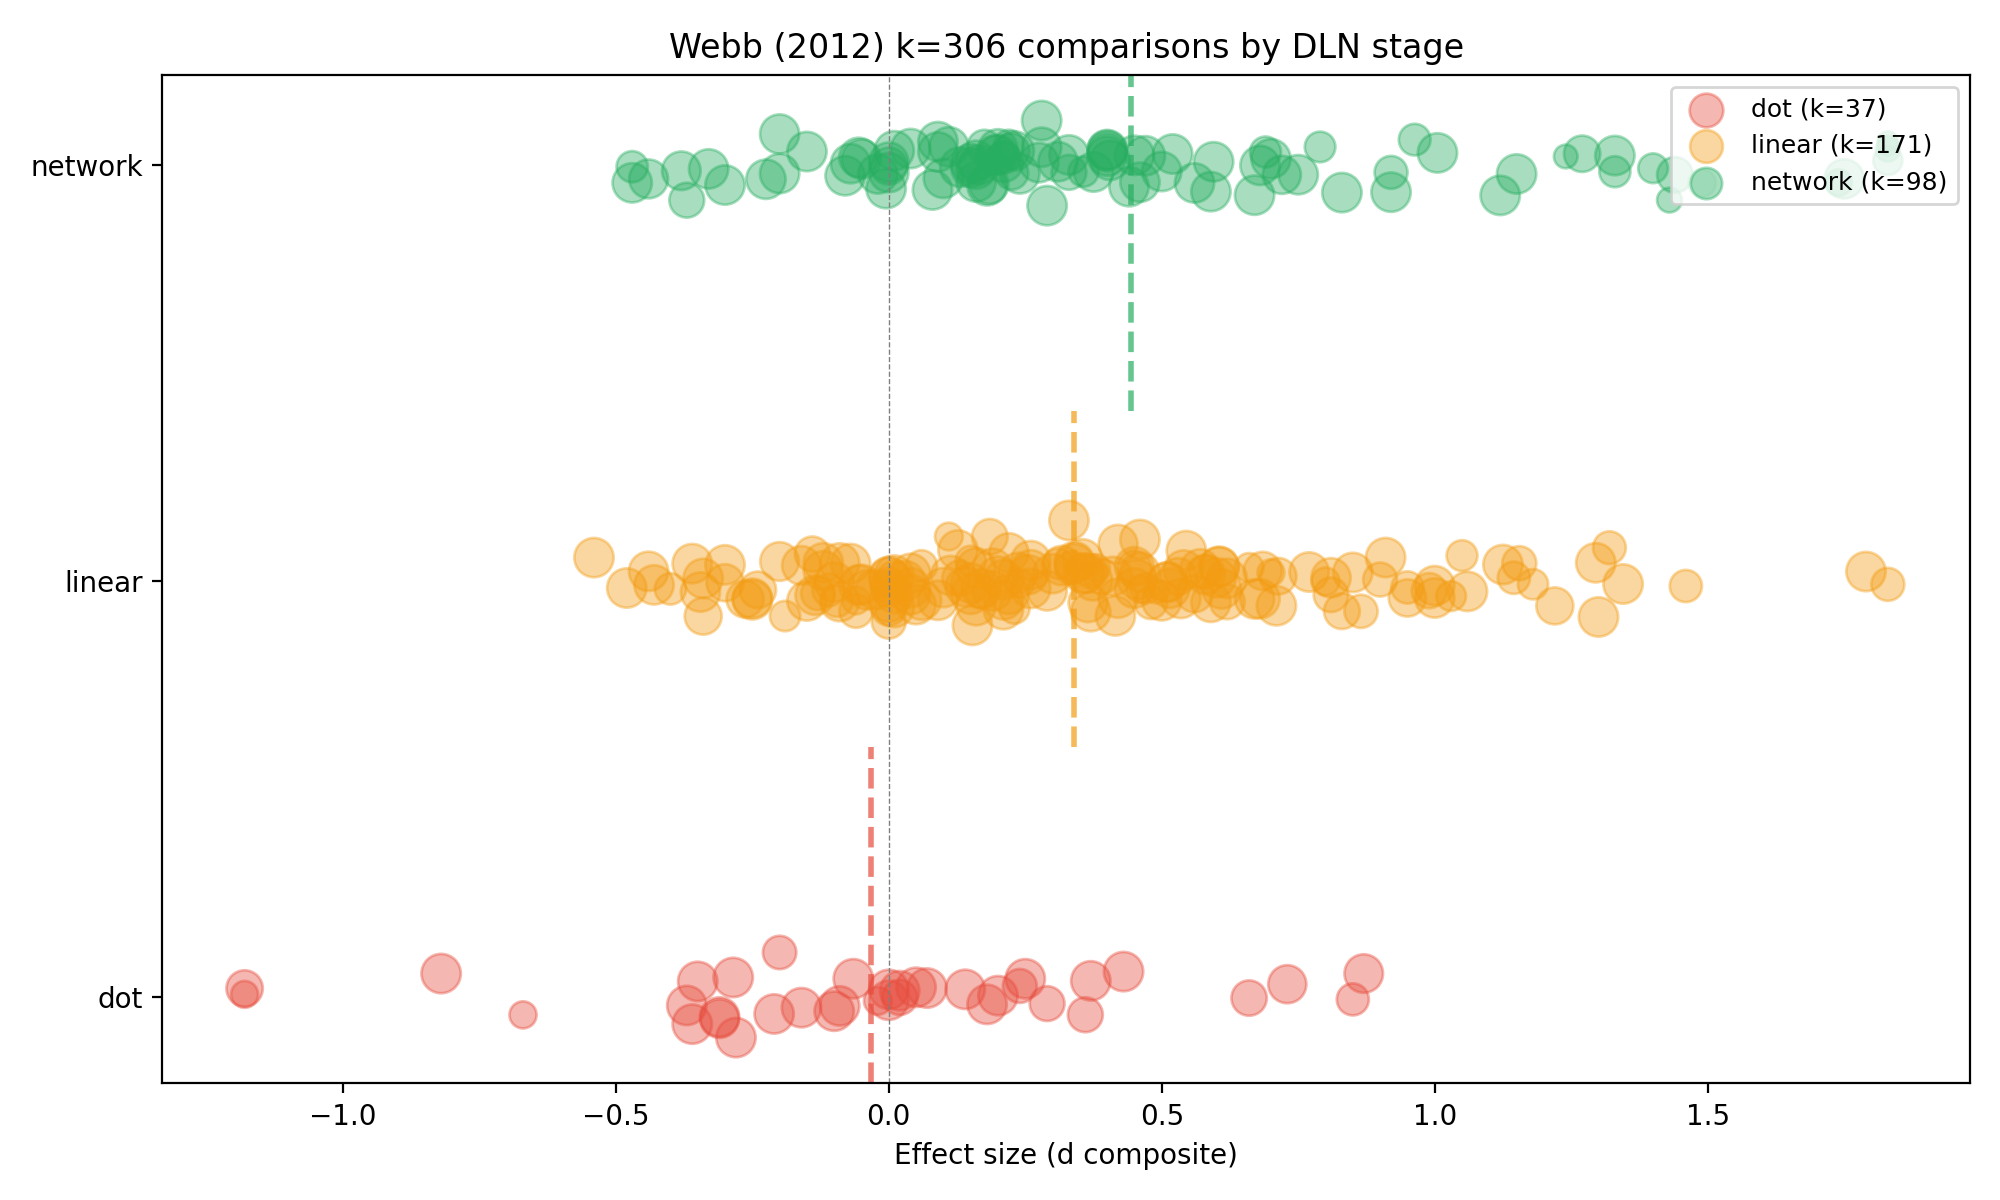
\includegraphics[width=0.85\linewidth]{../evidence_synthesis/outputs/figures/webb2012_full_forest_by_stage.png}
\caption{Forest plot of Webb et al.\ (2012) comparison-level effect
sizes ($k = 306$) grouped by DLN stage coding. Dot-stage strategies
(situation selection, concentration; $k = 37$) cluster near zero;
linear-stage strategies (distraction, suppression, situation
modification, other response modulation; $k = 171$) show intermediate
effects; network-stage strategies (reappraisal, perspective-taking,
other cognitive change, acceptance; $k = 98$) show the largest positive
regulation effects. The graded ordering is consistent with the DLN
framework's prediction that integrative architectures support more
effective emotion regulation.}
\label{fig:forest}
\end{figure}


\subsection{Permutation tests indicate DLN coding is non-arbitrary}

A key concern with small-$k$ moderator analyses is that any
sufficiently favourable partition might achieve comparable variance
reduction by chance (model saturation). We addressed this by conducting
exhaustive permutation tests for all four datasets with between-stage
variation (Table~\ref{tab:permutation}).

For the Webb anchor analysis, a Monte Carlo permutation test with
10{,}000 random three-way partitions of the 306 comparisons (preserving
group sizes 37, 171, 98) was conducted. For each partition, the same
REML meta-regression was fit and the residual $\hat\tau^2$ recorded
(Fig.~\ref{fig:perm}). The DLN-coded $\hat\tau^2$ (0.112) fell below
all 10{,}000 random partitions ($p < 0.001$; median random-partition
$\hat\tau^2 = 0.125$). At the aggregated strategy-family level
($k = 10$), an exhaustive enumeration of all $S(10,3) = 9{,}330$
unique partitions confirmed significance ($p = 0.025$).

We extended this approach to the three cross-domain datasets. The
interoception analysis ($S(8,3) = 966$ partitions) produced the
strongest result: DLN coding outperformed 99.8\% of random assignments
($p = 0.002$). The Hoyt health-psychology analysis ($S(8,3) = 966$)
was similarly significant ($p = 0.008$).

One analysis did not reach significance. The Desmedt HCT analysis
($S(7,2) = 63$ two-way partitions; $p = 0.111$) achieved a
large absolute $\hat\tau^2$ reduction (83\%) among the
cross-domain datasets, but with only 63 possible partitions the
minimum achievable $p$-value is $1/63 \approx 0.016$ and the test
has limited resolution; DLN coding still outperformed 89\% of random
assignments. We retain this analysis for its qualitative pattern
(same-level correspondence between HCT and biological criteria) while
noting that the individual permutation evidence is inconclusive.

Across the five datasets with between-stage variation, four of five
permutation tests were significant at $p < 0.05$ (three exhaustive,
two Monte Carlo with 10{,}000 draws; combined by Fisher's method:
$p < 0.001$). Because all five analyses share
a common coding framework and were coded by the same author, the
individual permutation $p$-values are not statistically independent;
the Fisher combined value is therefore best interpreted as a summary
statistic quantifying the overall pattern rather than a formal omnibus
test of independent replications (see Methods~M4).


\begin{table}[ht]
\centering
\small
\caption{Permutation tests for DLN stage coding across all five
datasets with between-stage variation. $S(n,k)$: Stirling number of
the second kind (number of unique partitions). The permutation
$p$-value is the proportion of all partitions achieving
$\hat\tau^2 \leq \hat\tau^2_{\text{DLN}}$. All enumerations were
exhaustive except Webb and Greenwald ($^\dagger$Monte Carlo,
10{,}000 draws).}\label{tab:permutation}
\begin{tabular}{lcccccc}
\toprule
\textbf{Analysis} & \textbf{$k$} & \textbf{Groups} & \textbf{Partitions}
& \textbf{DLN $\hat\tau^2$} & \textbf{Median perm.\ $\hat\tau^2$}
& \textbf{Perm.\ $p$} \\
\midrule
Webb\cite{Webb2012} & 306 & 3 & 10{,}000$^\dagger$ & 0.112 & 0.125 & $<$0.001 \\
Interoception & 8 & 3 & 966 & 0.021 & 0.143 & 0.002 \\
Hoyt\cite{Hoyt2024} & 8 & 3 & 966 & 0.000 & 0.039 & 0.008 \\
Desmedt\cite{Desmedt2022} & 7 & 2 & 63 & 0.000 & 0.002 & 0.111 \\
Greenwald\cite{Greenwald2009} & 184 & 4 & 10{,}000$^\dagger$ & 0.011 & 0.017 & $<$0.001 \\
\bottomrule
\end{tabular}
\end{table}


\begin{figure}[ht]
\centering
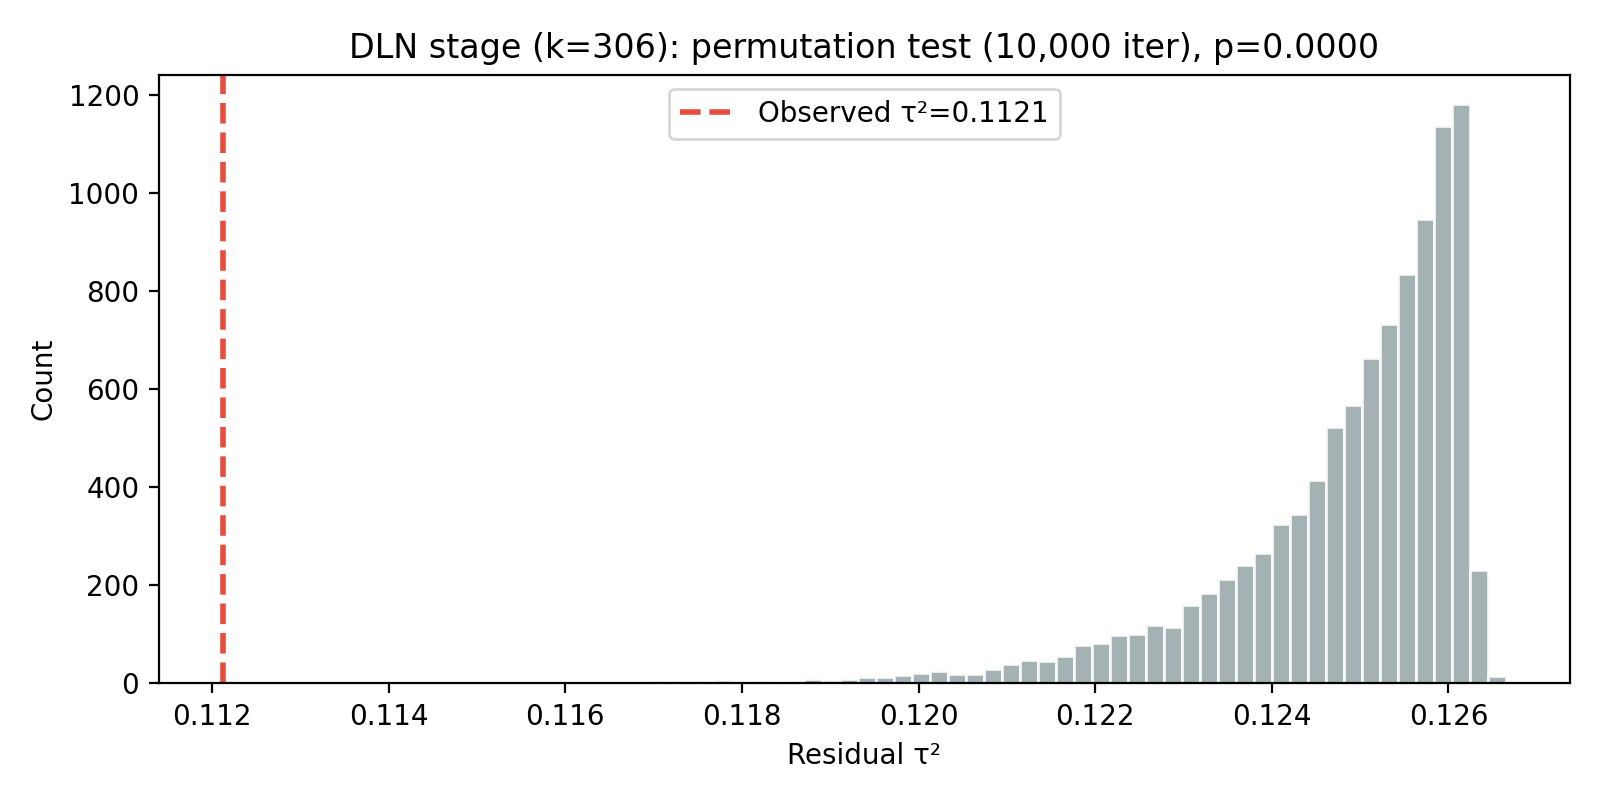
\includegraphics[width=0.85\linewidth]{../evidence_synthesis/outputs/figures/webb2012_full_permutation.png}
\caption{Permutation distribution of residual $\hat\tau^2$ across
10{,}000 random three-way partitions of the 306 Webb et al.\ (2012)
experimental comparisons (group sizes preserved). The dashed red line
marks the DLN-coded $\hat\tau^2 = 0.112$, which falls below all
random assignments ($p < 0.001$). At the aggregated strategy-family
level ($k = 10$), an exhaustive test ($S(10,3) = 9{,}330$ partitions)
confirmed significance ($p = 0.025$). Analogous tests for the three
cross-domain datasets are reported in Table~\ref{tab:permutation};
distribution plots are provided in the Supplementary Information.}
\label{fig:perm}
\end{figure}


\subsection{Cross-domain moderator analyses}

The Webb reanalysis demonstrates that DLN stage coding captures
meaningful variance within a single domain. To evaluate whether this
result generalises, we applied the same analytic approach---coding
published meta-analytic data for DLN stage and fitting random-effects
meta-regression---to three additional datasets spanning
interoception and health psychology
(Table~\ref{tab:cross_domain}; Methods~M6).

\paragraph{Interoception--alexithymia association.}
We synthesised interoceptive measure families ($k = 8$) from Trevisan et
al.\cite{Trevisan2019} and Van Bael et al.\cite{VanBael2024}, coding
each by processing architecture: dot (heartbeat detection tasks, body
awareness---raw signal detection), linear (interoceptive confusion,
autonomic reactivity, EDI interoceptive awareness---single-dimension
distress tracking), and network (Interoceptive Accuracy Scale, MAIA,
Body Awareness Questionnaire---multi-dimensional integrative awareness).
DLN stage coding reduced $\hat\tau^2$ from 0.134 ($I^2 = 99.6\%$) to
0.021 ($I^2 = 95.6\%$), an 84.7\% reduction ($Q_M(2) = 1700.03$,
$p < 0.001$; permutation $p = 0.002$; Table~\ref{tab:permutation}). Critically, the moderator
coefficients revealed a \textit{sign reversal}: relative to dot
(intercept $= -0.04$), linear-stage measures showed a large positive
shift ($b = 0.48$, 95\% CI $[0.13, 0.82]$) and network-stage measures a
negative shift ($b = -0.27$, 95\% CI $[-0.62, 0.07]$). That is,
linear-coded interoceptive measures (confusion, reactivity) correlate
\textit{positively} with alexithymia, while network-coded measures
(MAIA, IAS) correlate \textit{negatively}---a qualitative shift in the
direction of the relationship depending on DLN stage
(Fig.~\ref{fig:cross_domain}a).

\paragraph{Heartbeat counting task criterion validity (Desmedt et al.,
2022).}
Desmedt et al.\cite{Desmedt2022} reported associations between heartbeat
counting task (HCT) performance and seven criterion measures ($k = 7$).
Because HCT is a dot-stage task (raw cardiac signal detection), DLN
predicts stronger associations with same-level criteria (biological
measures) than with cross-level criteria (psychological self-report).
We coded criteria as dot (heart rate, BMI, age, sex---biological) or
linear (trait anxiety, depression, alexithymia---self-report). Using
absolute $|r|$ as the dependent variable, DLN stage coding reduced
$\hat\tau^2$ from 0.002 ($I^2 = 54.3\%$) to 0.000 ($I^2 = 2.6\%$),
an 82.6\% reduction ($Q_M(1) = 7.99$, $p = 0.005$;
permutation $p = 0.111$; Table~\ref{tab:permutation}). The dot coefficient was positive ($b = 0.10$,
95\% CI $[-0.00, 0.20]$), with the confidence interval marginally
including zero under the Knapp--Hartung adjustment ($df = 5$):
dot-stage criteria showed stronger associations with HCT performance
than linear-stage criteria (dot mean $|r| = 0.13$, linear mean
$|r| = 0.03$), supporting the same-level correspondence prediction
at the level of point estimates.

\paragraph{Emotional approach coping and health (Hoyt et al., 2024).}
Hoyt et al.\cite{Hoyt2024} meta-analysed the association between
emotional approach coping (EAC) and health outcomes across domains ($k = 8$
outcome families; all domain-level $r$ values verified from Table~3).
We coded outcome domains by the structural features of their
measurement instruments: dot (biological/physiological, physical health,
behavioural---single-modality somatic outcomes), linear (mental/emotional
distress, risk-related adjustment---unidimensional symptom severity
measures), and network (positive psychological health,
social functioning, resilience/benefit-finding---multi-domain
integrative appraisals). DLN stage coding reduced $\hat\tau^2$ from 0.038
($I^2 = 93.3\%$) to 0.000 ($I^2 = 0\%$), a 100\% reduction ($Q_M(2) = 102.36$, $p < 0.001$;
permutation $p = 0.008$; Table~\ref{tab:permutation}). The moderator
coefficients revealed a pattern consistent with the
\textit{dangerous-middle} prediction (Fig.~\ref{fig:cross_domain}b):
relative to the dot-stage intercept ($b = 0.02$, 95\% CI $[-0.09,
0.14]$), linear-coded domains showed a significant \textit{negative}
shift ($b = -0.16$, 95\% CI $[-0.30, -0.01]$), while network-coded
domains showed a large positive shift ($b = 0.28$, 95\% CI $[0.14,
0.42]$). That is, emotional approach coping is associated with worse
outcomes precisely in linear-coded domains---where emotion is processed
as interference under compartmentalisation---while producing near-zero
effects in dot-coded domains and strongly positive effects in
network-coded domains. This V-shaped pattern, in which partial
integration produces worse outcomes than either reactive responding or
full integration, is the empirical signature of the dangerous-middle
prediction derived from the DLN computational framework\cite{Wu2026}.


\begin{table}[ht]
\centering
\small
\caption{Cross-domain moderator analyses. All analyses used
random-effects meta-regression (REML, Knapp--Hartung adjustment) with
DLN stage as a categorical moderator. $\Delta\hat\tau^2$: reduction in
residual heterogeneity relative to the intercept-only baseline. Analyses
are ordered by domain. Egger's test was non-significant in all analyses.
All effect sizes are verified from published source
tables (see Methods~M6).}\label{tab:cross_domain}
\begin{tabularx}{\linewidth}{p{0.14\linewidth} p{0.11\linewidth}
  >{\centering\arraybackslash}p{0.03\linewidth}
  >{\centering\arraybackslash}p{0.05\linewidth}
  >{\centering\arraybackslash}p{0.06\linewidth}
  >{\centering\arraybackslash}p{0.06\linewidth}
  >{\centering\arraybackslash}p{0.06\linewidth}
  >{\centering\arraybackslash}p{0.08\linewidth}
  >{\centering\arraybackslash}p{0.06\linewidth}
  X}
\toprule
\textbf{Meta-analysis} & \textbf{Domain} & \textbf{$k$} &
\textbf{Unit} & \textbf{Base $\hat\tau^2$} & \textbf{DLN $\hat\tau^2$}
& \textbf{$\Delta\hat\tau^2$} & \textbf{$Q_M$ ($p$)} & \textbf{Perm.\ $p$}
& \textbf{Key pattern} \\
\midrule
Webb\cite{Webb2012}$^a$ & Emotion reg. & 10 & Strategy & 0.035 &
0.011 & 70\% & 30.0 ($<$0.001) & 0.025 & Network $>$ Lin.\ $>$ Dot \\[3pt]
Trevisan; Van Bael\cite{Trevisan2019, VanBael2024} & Interoception &
8 & Measure & 0.134 & 0.021 & 85\% & 1700.0 ($<$0.001) & 0.002 & Sign reversal \\[3pt]
Desmedt\cite{Desmedt2022} & HCT validity & 7 & Criterion &
0.002 & 0.000 & 83\% & 8.0 (0.005) & 0.111 & Same $>$ cross-level \\[3pt]
Hoyt\cite{Hoyt2024} & Health psych. & 8 & Domain & 0.038
& 0.000 & 100\% & 102.4 ($<$0.001) & 0.008 & V-shape \\[3pt]
Greenwald\cite{Greenwald2009} & Implicit cog. & 184 & Study &
0.017 & 0.011 & 32.9\% & 141.0 ($<$0.001) & $<$0.001 & Suppression \\[3pt]
Zanini\cite{Zanini2025} & Affect.\ decision & 110 & Study & --- & ---
& N/A & --- & --- & Boundary: all dot \\
\midrule
\multicolumn{10}{l}{\footnotesize $^a$Comparison-level analysis ($k = 306$, 190 studies) confirms: $Q_M(2) = 54.01$, $p < 0.001$; cluster-robust $p < 0.001$; Monte Carlo perm.\ $p < 0.001$.} \\
\bottomrule
\end{tabularx}
\end{table}


\subsection{Implicit cognition: Greenwald et al.\ (2009)}

Greenwald et al.\cite{Greenwald2009} reported IAT predictive validity
across criterion domains ($k = 184$ independent samples, $N \approx
14{,}900$). Domain-level coding (consumer = dot, intergroup = linear,
relationships = network) assumes homogeneous processing within domains,
but the same domain can contain criterion behaviours at different DLN
levels---for example, race-related physiological responses (amygdala
activation, startle blink) are reactive (dot), whereas deliberative
intergroup discrimination under social-desirability pressure reflects
externally imposed normative structure (linear-plus in the compression
model's terminology\cite{Wu2026}). We therefore coded all 184 samples
at the study level based on the criterion behaviour's representational
topology: dot ($k = 33$; reflexive, physiological, or automatic
criteria), linear ($k = 97$; independent option evaluations without
normative constraint), linear-plus ($k = 43$; deliberative intergroup
behaviour under social-desirability pressure), and network ($k = 11$;
political behaviour connected through latent ideological structure).

Three-level DLN coding (collapsing linear-plus into linear: dot $k = 33$,
linear $k = 140$, network $k = 11$) reduced ICC heterogeneity by 29.6\%
($\hat\tau^2$: 0.017 $\to$ 0.012; $Q_M(2) = 129.7$, $p < 0.001$),
preserving the network $>$ dot $>$ linear ordering ($\bar{r} = 0.46$,
$0.32$, $0.25$). Distinguishing linear-plus from linear (four-level
coding) further reduced heterogeneity to 32.9\%
($\hat\tau^2$: 0.017 $\to$ 0.011; $I^2$: 65.4\% $\to$ 53.5\%;
$Q_M(3) = 141.0$, $p < 0.001$; Table~\ref{tab:cross_domain}). Adding
criterion-aggregation covariates ($n_\mathrm{crit}$, $n_\mathrm{IAT}$)
increased reduction to 48.9\%.
A Monte Carlo permutation test (10{,}000 random four-way partitions
with matched group sizes) confirmed that no random partition achieved
equal or lower residual $\hat\tau^2$ ($p < 0.001$). Network-coded
samples showed the highest ICC ($\bar{r} = 0.47$), followed by dot
(0.34), linear (0.27), and linear-plus (0.23).

The four-level coding reveals a suppression fingerprint: linear-plus
samples showed the lowest implicit--explicit correlation
($\overline{\mathrm{iec}} = 0.199$) and the only positive ICC--ECC gap
among deliberative stages ($+0.050$), consistent with the compression
model's prediction that externally imposed normative structure
suppresses explicit expression while leaving implicit associations
intact\cite{Wu2026}. Network-coded samples showed the highest
implicit--explicit correlation ($\overline{\mathrm{iec}} = 0.521$) and
the highest absolute validity across both measurement channels (ICC and
ECC), consistent with shared latent-factor structure being accessible
to both implicit and explicit processing.
This suppression fingerprint was robust to coding decisions: across 31
alternative codings that toggled the five most debatable boundary
assignments between linear and linear-plus, $\hat\tau^2$ reduction
ranged from 28.7\% to 34.7\%, and linear-plus showed the lowest iec in
all 31 scenarios.
The 184 samples span nine topic domains (Consumer, Race, Clinical,
Drugs/tobacco, Personality, Gender/sex, Other intergroup,
Relationships, Politics), and samples within domains share both
stage assignment and substantive content. The effective $k$ for
between-stage tests is therefore closer to 9 than to 184.
The study-level permutation test above does not address this
clustering. To do so, we conducted an exhaustive domain-level
permutation test: all $S(9,4) = 7{,}770$ unique partitions of the
9 domains into 4 non-empty groups were enumerated, constraining
every study within a domain to the same group. The DLN
domain-to-stage mapping outperformed 95.9\% of all possible
domain-level assignments ($p = 0.041$), confirming that the
four-level coding captures non-random structure even at the honest
effective $k = 9$.


\subsection{Zanini et al.\ (2025): boundary-condition test}

A framework's scope is sharpened by cases where it predicts no effect.
Zanini et al.\cite{Zanini2025} provides a pre-registered boundary test. This
meta-analysis of Iowa Gambling Task sex differences ($k = 110$) included
exclusively standard 100-trial IGT studies with healthy naive
participants. Application of our pre-specified coding rubric assigned
every study to dot stage, yielding no between-stage variation.

DLN stage requires between-stage variation to function as a moderator.
When all studies occupy a single stage, the theory predicts
$\hat\tau^2$ reduction $= 0\%$. Zanini et al.\ tested seven moderators
and found none significant---consistent with the prediction that
within-stage heterogeneity ($Q(109) = 206$, $\hat\tau^2 = 20.8$)
reflects sources that architectural coding is not designed to capture.
The contrast between the positive moderator results above and this
null is consistent with DLN generating discriminating predictions with
identifiable boundary conditions, though a single null result
cannot rule out alternative explanations for the absence of moderation.


\subsection{Competing moderator analysis}

A key question is whether DLN stage coding provides explanatory value
beyond simpler, atheoretical alternatives. For each primary dataset,
we defined 2--3 alternative moderator codings grounded in established
taxonomies or obvious structural features, fit the same REML
meta-regression, and compared $\hat\tau^2$ reduction, AICc, and
permutation $p$-values (Table~\ref{tab:competing}).

DLN stage achieved the highest $\hat\tau^2$ reduction in all four
datasets: 70\% vs.\ 23\% for cognitive effort in Webb (at the
strategy-family level; the comparison-level analysis yielded 10\% vs.\
1.8\%, with the best AICc among all moderators); 85\% vs.\ 24\%
for the next-best alternative (emotion--body link) in interoception;
100\% vs.\ 71\% for temporal frame in Hoyt; and 83\% tied with
measurement objectivity in Desmedt. Importantly, the Desmedt tie
is expected: the measurement-objectivity coding (objective vs.\
self-report) is \textit{exactly equivalent} to the DLN coding
(biological vs.\ psychological) for this dataset, confirming that
DLN stage captures a meaningful structural distinction. The Gross
process model---the most established alternative for Webb---in fact
\textit{increased} heterogeneity ($-17\%$), consistent with Webb et
al.'s\cite{Webb2012} original finding that the process-model
taxonomy does not predict strategy effectiveness.

DLN did not achieve the lowest AICc in three of four datasets, because
AICc penalises additional parameters and several alternatives use only
two levels. This is an inherent parsimony trade-off: DLN's three-level
coding uses more degrees of freedom but captures qualitative sign
patterns (V-shape, sign reversal) that two-level alternatives cannot
represent.


\begin{table}[ht]
\centering
\small
\caption{Competing moderator analysis: DLN stage vs.\ alternative
codings. For each dataset, the same REML meta-regression was fit with
each moderator. $\Delta\hat\tau^2$: percentage reduction from the
intercept-only baseline. $Q_M$: omnibus moderator test with $p$-value.
AICc: small-sample corrected Akaike criterion
(lower is better). Perm.\ $p$: exhaustive permutation
$p$-value. The best $\hat\tau^2$ reduction per dataset is
\textbf{bolded}.}\label{tab:competing}
\begin{tabular}{llcrrrrc}
\toprule
\textbf{Dataset} & \textbf{Moderator} & \textbf{Levels} &
\textbf{$\Delta\hat\tau^2$} & \textbf{$Q_M$ ($p$)} & \textbf{AICc} &
\textbf{Perm.\ $p$} \\
\midrule
Webb & \textbf{DLN stage} & 3 & \textbf{70\%} & 30.0 ($<$0.001) & $-0.8$ & 0.025 \\
 & Cognitive effort & 2 & 23\% & 12.7 (${<}0.001$) & $-5.1$ & 0.145 \\
 & Gross process model & 2 & $-17\%$ & 2.6 (0.105) & $-2.9$ & 0.988 \\
\midrule
Interoception & \textbf{DLN stage} & 3 & \textbf{85\%} & 1700.0 ($<$0.001) & 10.2 & 0.002 \\
 & Garfinkel trichotomy & 3 & $-22\%$ & 229.1 (${<}0.001$) & 20.1 & 0.726 \\
 & Measurement method & 2 & $-16\%$ & 9.3 (0.002) & 8.8 & 0.874 \\
 & Emotion--body link & 2 & 24\% & 858.0 ($<$0.001) & 7.2 & 0.118 \\
\midrule
Hoyt & \textbf{DLN stage} & 3 & \textbf{100\%} & 102.4 ($<$0.001) & $-0.5$ & 0.008 \\
 & Construct valence & 2 & 63\% & 74.8 ($<$0.001) & $-3.0$ & 0.055 \\
 & Meas.\ dimensionality & 2 & 56\% & 72.5 ($<$0.001) & $-1.4$ & 0.063 \\
 & Temporal frame & 2 & 71\% & 78.3 ($<$0.001) & $-4.4$ & 0.039 \\
\midrule
Desmedt & \textbf{DLN stage} & 2 & \textbf{83\%} & 8.0 (0.005) & $-9.7$ & 0.111 \\
 & Meas.\ objectivity & 2 & 83\% & 8.0 (0.005) & $-9.7$ & 0.111 \\
 & Clinical relevance & 2 & $-35\%$ & 0.1 (0.709) & $-5.6$ & 0.825 \\
\bottomrule
\end{tabular}
\end{table}


\begin{figure}[ht]
\centering
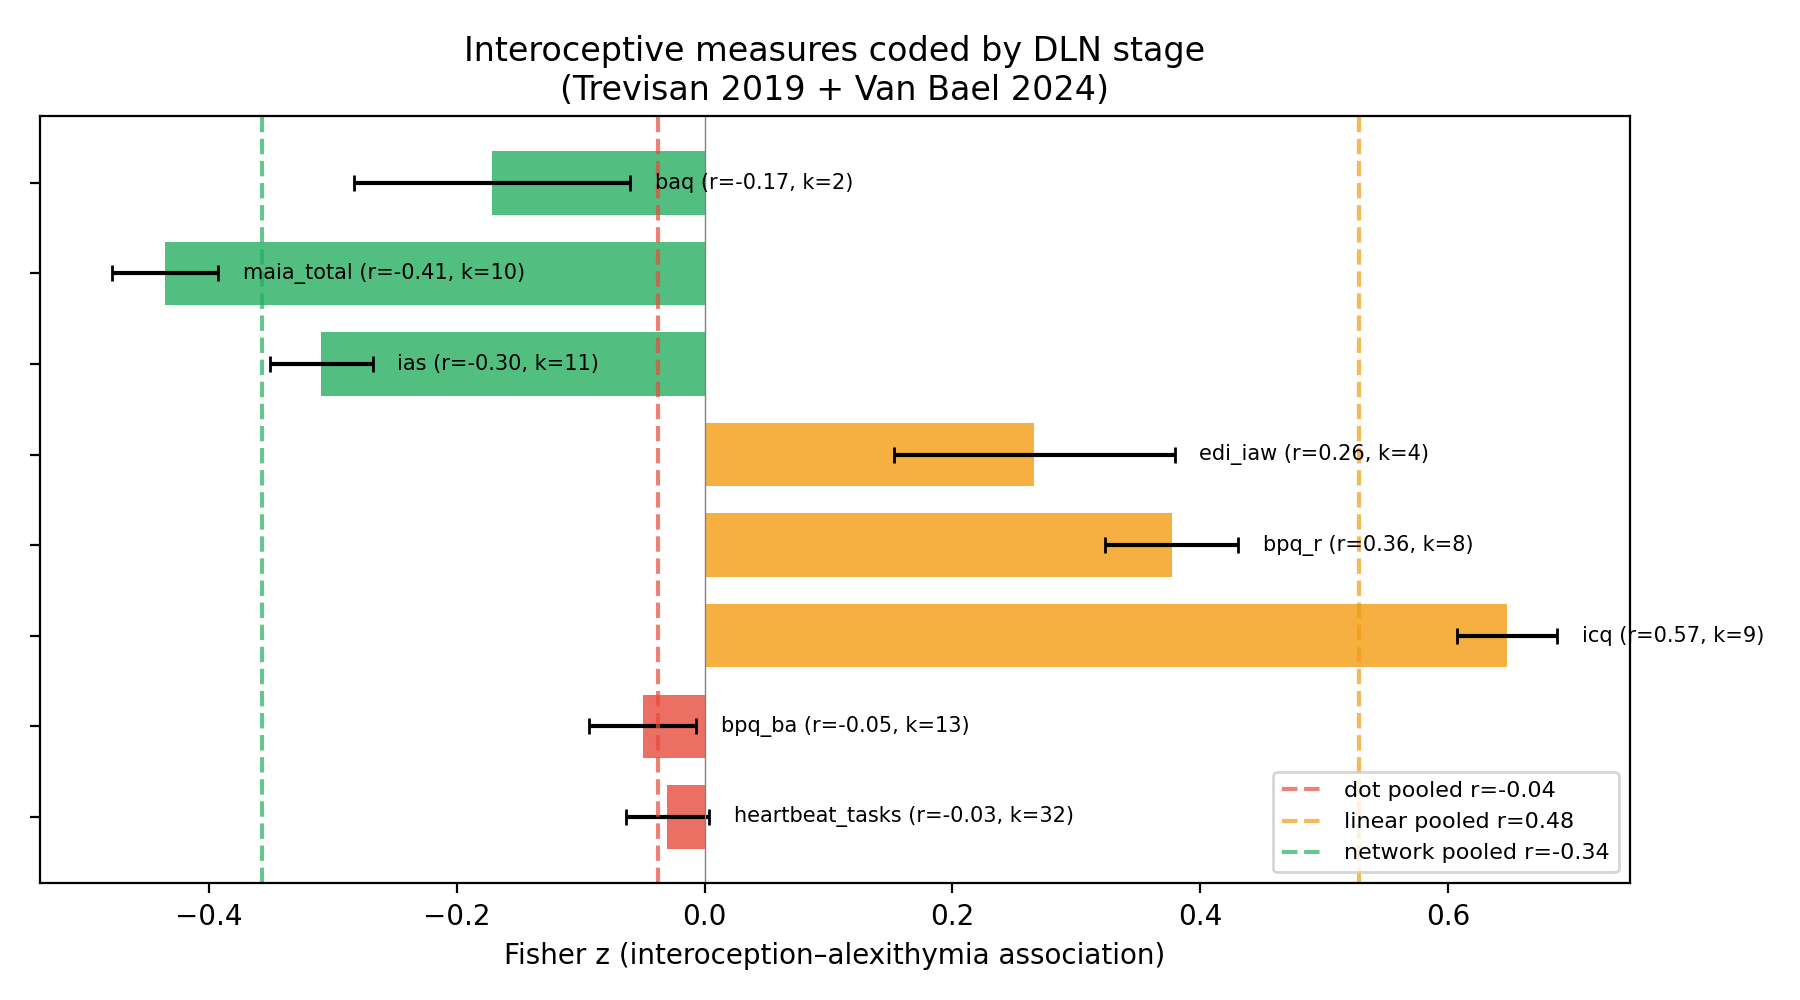
\includegraphics[width=0.48\linewidth]{../evidence_synthesis/outputs/figures/interoception_stage_forest.png}%
\hfill
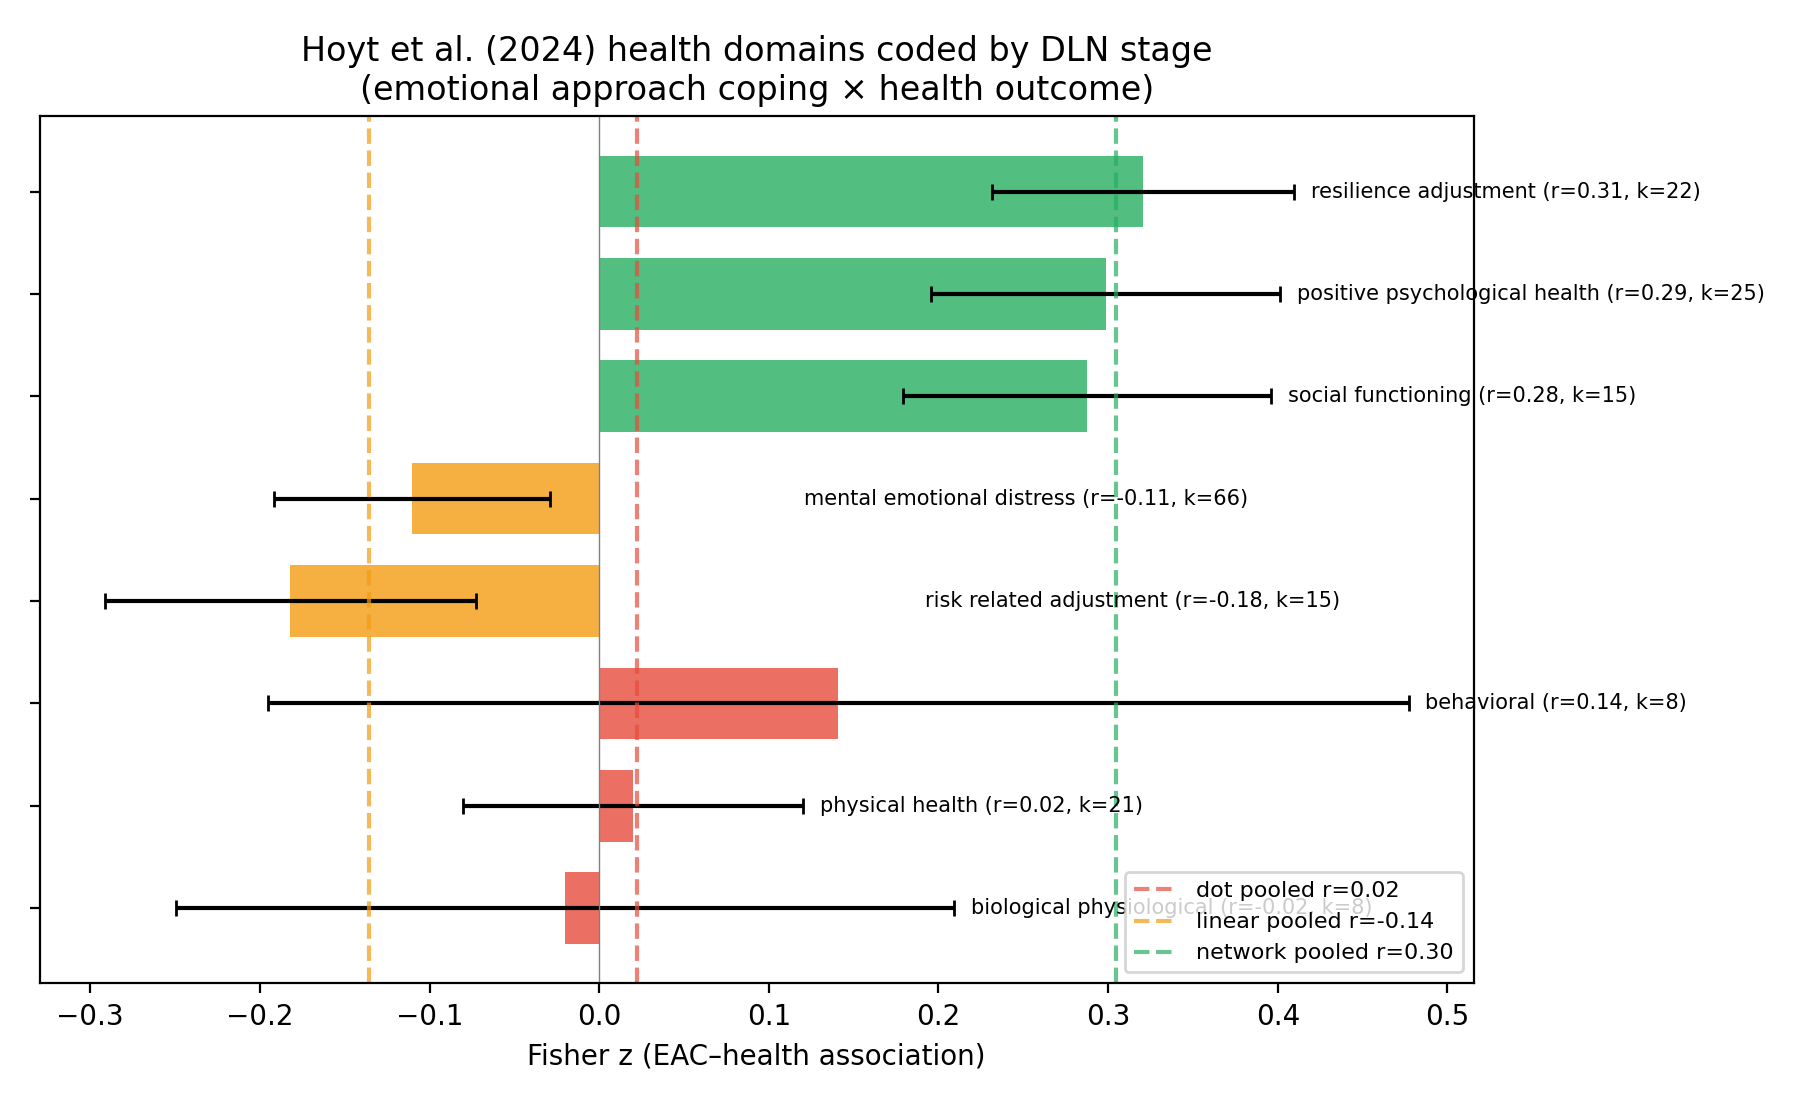
\includegraphics[width=0.48\linewidth]{../evidence_synthesis/outputs/figures/hoyt2024_stage_forest.png}
\caption{Two diagnostic patterns from cross-domain moderator analyses.
\textbf{(a)}~Interoception--alexithymia: sign reversal by DLN stage.
Linear-coded measures (confusion, reactivity) correlate positively
with alexithymia; network-coded measures (MAIA, IAS) correlate
negatively. Dot-coded measures (heartbeat tasks) are near zero.
\textbf{(b)}~Emotional approach coping and health (Hoyt et al.):
dangerous-middle V-shape. Dot- and network-coded domains show positive
effects; linear-coded domains (mental distress, risk-related
adjustment) show negative effects, consistent with the prediction that
partial integration without metacognitive monitoring produces worse
outcomes than full compartmentalisation.}
\label{fig:cross_domain}
\end{figure}


\subsection{Summary of cross-domain predictions: supported and
prospective}

The five moderator analyses and one boundary condition permit a status
assessment of the DLN framework's cross-domain predictions:

\begin{enumerate}[nosep]
\item \textit{Heterogeneity reduction} (supported): At the
strategy/measure/domain level, DLN stage coding reduces $\hat\tau^2$
by 70--100\% in all four category-level datasets with between-stage
variation (Webb $k = 10$, interoception, Desmedt, Hoyt). The
comparison-level Webb analysis ($k = 306$, 190 studies) confirms the
moderator with higher statistical power ($Q_M = 54.01$, $p < 0.001$;
cluster-robust $p < 0.001$; Monte Carlo permutation $p < 0.001$).
Study-level four-level coding of the Greenwald dataset ($k = 184$)
reduces $\hat\tau^2$ by 32.9\%; remaining within-stage variance
reflects criterion-quality noise (covariates raise reduction to
48.9\%). Permutation tests were significant in four of five datasets
($p < 0.001$).
\item \textit{Directional ordering} (supported): Network-coded effects
exceed linear-coded effects in the predicted direction across five
domains---higher regulation effectiveness (Webb), tighter
body--emotion coupling (interoception), stronger same-level
correspondence (Desmedt), more adaptive health outcomes (Hoyt), and
higher criterion validity with greater implicit--explicit alignment
(Greenwald).
\item \textit{Dangerous-middle prediction} (supported): Hoyt et al.\
show that linear-coded domains produce significantly worse outcomes
than dot-coded domains ($b = -0.16$, 95\% CI $[-0.30, -0.01]$),
while network-coded domains show strongly positive effects ($b = 0.28$,
95\% CI $[0.14, 0.42]$), consistent with the DLN computational
prediction that partial integration without metacognitive monitoring
amplifies rather than mitigates risk.
\item \textit{Boundary conditions} (supported): Zanini ($k = 110$,
all dot) correctly predicts null moderation.
\end{enumerate}

\noindent A more granular set of predictions specifying particular
measures and expected effect patterns is provided in Supplementary
Table~1.


\subsection{Deposited empirical protocol: cumulative exposure
sensitivity}

The analyses above code task and measure characteristics; they do not
classify individual participants. We deposit a preregistered protocol
for an individual-level test of the dangerous-middle prediction: a
stage $\times$ cumulative exposure interaction in which DLN stage is
assessed via independent structural representation tasks and cumulative
emotional consequences build over trials\cite{Wu2026}. The full protocol,
including sample size justification, randomisation scheme, and analysis
plan, is deposited at:
\texttt{empirical\_tests/protocol/cumulative\_exposure\_protocol.md}.


\section{Discussion}

Across five moderator analyses spanning four domains of psychology,
DLN stage coding reduced meta-analytic heterogeneity by 70--100\% in
four datasets, produced theoretically predicted sign reversals and
directional orderings in five, and correctly predicted null moderation
in a boundary-condition dataset (Table~\ref{tab:cross_domain}). These
results provide converging evidence that cognitive architecture---the
topology of the belief-dependency graph through which information is
processed---functions as a hidden structural moderator of empirical
relationships that conventional moderators leave unexplained.

The anchor result remains the Webb et al.\cite{Webb2012} reanalysis.
At the comparison level ($k = 306$), DLN stage coding was the
strongest moderator ($Q_M(2) = 54.01$, $p < 0.001$; cluster-robust
$p < 0.001$; Monte Carlo permutation $p < 0.001$), reducing
between-comparison heterogeneity by 10\%. When aggregated to the
strategy-family level ($k = 10$), the same coding reduced
between-strategy heterogeneity by 70\% (exhaustive permutation
$p = 0.025$). An important question is whether DLN stage
coding merely relabels Webb et al.'s existing process-model
taxonomy\cite{Gross2002}. Three observations argue against this
interpretation. First, the mapping is not one-to-one: DLN recodes
\textit{across} Gross families (e.g., acceptance is response modulation
in the process model but network in DLN; concentration is attentional
deployment in the process model but dot in DLN). Second, the process
model's temporal ordering prediction was disconfirmed by Webb et al.'s
data, whereas DLN's compression-based ordering correctly predicts the
empirical pattern. Third, and most critically, DLN stage generalises
beyond emotion regulation to interoception, health psychology (Hoyt),
and implicit cognition (Greenwald)---domains for which the Gross
process model was not designed.

The dangerous-middle prediction receives domain-level evidence
consistent with the DLN framework from the Hoyt et
al.\cite{Hoyt2024} reanalysis. Conventional wisdom assumes that
greater emotional awareness uniformly improves outcomes. The DLN
framework instead predicts that partial integration---relational
emotional knowledge without metacognitive monitoring---can produce worse
outcomes than full compartmentalisation. This prediction follows from
the computational result that factor-level exploitation in the absence
of cumulative exposure tracking amplifies rather than mitigates
risk\cite{Wu2026}. The Hoyt data are consistent with this pattern:
emotional approach coping is associated with significantly worse
outcomes in linear-coded health domains ($b = -0.16$, 95\% CI
$[-0.30, -0.01]$) while producing near-zero effects in dot-coded
domains and strongly positive effects in network-coded domains
($b = 0.28$, 95\% CI $[0.14, 0.42]$). This V-shaped pattern is a direction-specific
prediction not generated by Levels of Emotional
Awareness\cite{Lane1987}, constructionist emotion
theory\cite{Barrett2017}, integrative complexity\cite{Suedfeld1976,
Tetlock1983}, or Acceptance and Commitment Therapy\cite{Hayes2006}.
The qualitative prediction that partial awareness without regulation
worsens outcomes has clinical precedent (insight without behavioural
change in OCD and psychosis, emotional processing without regulation
in complex PTSD); the DLN contribution is the computational
mechanism---cross-term catastrophe under factor-level exploitation
without exposure tracking---not the qualitative direction alone.
We note that the domain-level analysis tests whether \textit{outcome
categories} whose measurement reflects linear-stage processing show
systematically worse effects; the stronger individual-level version
of the dangerous-middle prediction---that partial integration (assessed
via independent structural tasks) produces worse outcomes under
cumulative load than full compartmentalisation---requires the
experimental test described in Section~2.7.
The interoception sign reversal provides complementary evidence:
linear-coded interoceptive measures correlate positively with
alexithymia while network-coded measures correlate negatively,
indicating that the same construct---interoceptive processing---relates
to emotion recognition deficits in opposite directions depending on
DLN stage.

The Greenwald et al.\cite{Greenwald2009} results merit candid
discussion. Study-level four-level coding reduced ICC heterogeneity by
32.9\%, substantially more than domain-level coding (1.5\%). This
improvement is itself informative: it demonstrates that DLN stage is a
property of the criterion behaviour's representational topology, not of
the domain category---a direct prediction of the compression model.
The 32.9\% reduction is lower than the 70--100\% observed in the
small-$k$ analyses because study-level data introduces substantial
within-stage criterion noise---variation in criterion aggregation
practices, sample composition, and IAT administration that the
four-level coding does not capture. This interpretation is supported
by the progressive reduction when covariates controlling criterion
specifics are added ($n_\mathrm{crit}$ and $n_\mathrm{IAT}$: 48.9\%).
The linear-plus category (intergroup discrimination under
social-desirability pressure) showed the predicted suppression
fingerprint: lowest implicit--explicit correlation and lowest explicit
criterion validity, consistent with externally imposed normative
structure suppressing explicit expression while leaving implicit
associations intact. The distinction between linear (independent
evaluation) and linear-plus (norm-governed evaluation) is formally
grounded in the compression model's definition of ``designer-specified
structure''\cite{Wu2026}, though its application to the Greenwald data
is post-hoc relative to the three-level study-level coding. The
sensitivity analysis (31 alternative codings) confirms robustness.
Importantly, the Greenwald analysis differs from the small-$k$
analyses in unit of analysis: the 184 samples span nine domain
categories, and the effective $k$ for between-stage tests is closer
to 9 than to 184; the domain-level permutation test ($p = 0.041$;
see Results) confirms the coding is non-arbitrary at this effective
sample size. Network-coded samples ($k = 11$) are exclusively
political behaviour, limiting generalisability of the network-stage
estimate.

Several limitations qualify these results. First, all codings except
the Zanini rubric were initially performed by the author with
knowledge of the DLN framework. To address this directly, two
independent coders naive to the DLN framework applied the deposited
rubrics to blinded extraction data for the Webb ($k = 10$), Hoyt
($k = 8$), and Greenwald topic-level ($9$ domains) datasets.
Inter-rater agreement was perfect for Hoyt
($\kappa = 1.000$, 8/8 items), and consensus codes matched the
author's original codes for all 27 items across three datasets
(Methods~M10). Four additional safeguards reinforce this result.
(a)~Exhaustive permutation tests assess
whether any arbitrary grouping achieves comparable variance
reduction, testing directly whether DLN coding captures non-random
structure (four of five datasets significant, $p < 0.001$--$0.025$;
Fisher's combined $p < 0.001$). (b)~A systematic coding sensitivity
analysis identifies the 2--5 most debatable stage assignments in each
dataset and reruns all analyses under every plausible alternative
coding (Webb: 8 strategy-family scenarios and 4 comparison-level
scenarios; interoception: 4; Hoyt: 4; Greenwald: 31 scenarios); the
qualitative sign pattern was preserved in 47/47 strategy-family
scenarios, and the
comparison-level Webb analysis remained significant ($Q_M$ range
32--54, all $p < 0.001$) in all 4 boundary scenarios
(Supplementary Table~2). (c)~All coding rationales are based on structural features
of measures and tasks (dimensionality, presence of relational
integration requirements, single- vs.\ multi-domain assessment), not
on observed effect directions. (d)~A competing moderator analysis
(Table~\ref{tab:competing}) compared DLN against 2--3 alternative
codings per dataset (Gross process model, cognitive effort, Garfinkel
trichotomy, construct valence, and others); DLN achieved the highest
$\hat\tau^2$ reduction in all four datasets. Crucially, none of the
alternative codings generalised across domains: moderators that
performed well in one dataset (e.g., temporal frame in Hoyt, 71\%)
failed in others, whereas DLN achieved $\geq$70\% reduction in every
dataset. This cross-domain consistency is the primary evidence that DLN
captures a structural variable rather than a domain-specific
distinction. An AI-assisted rubric consistency check provided
convergent evidence (Methods~M10). These safeguards address different
threats: permutation tests guard against arbitrary grouping,
sensitivity analyses guard against debatable boundary cases,
structural rationales guard against outcome-informed coding, and
competing moderator comparisons guard against the possibility that
any reasonable grouping would work equally well.
Blinded human coding was conducted for Webb, Hoyt, and the Greenwald
topic-level mappings (9 domains); two independent coders agreed with
author coding on all items (27/27 across three datasets). Independent
blinded coding of the interoception dataset remains a target for
future work.
Second, the cross-domain analyses operate at small $k$
(7--10 units); the comparison-level Webb analysis ($k = 306$) addresses
this concern for the anchor dataset, but the remaining category-level
analyses remain small-$k$. The 100\% $\hat\tau^2$ reduction in Hoyt
should be interpreted cautiously: with three parameters fitting 8 data
points,
model saturation contributes to apparent perfect fit. Profile-likelihood
confidence intervals\cite{Viechtbauer2010} for moderator $\hat\tau^2$
confirm wide parameter uncertainty at small $k$: for example, the Hoyt
moderator 95\% CI includes zero ($[0.000, 0.007]$), consistent with
near-complete heterogeneity reduction but substantial estimation
uncertainty. Two complementary safeguards address this concern. Exhaustive permutation
tests assess whether any arbitrary grouping achieves comparable
variance reduction; three of four small-$k$ datasets were significant
($p = 0.002$--$0.025$; Table~\ref{tab:permutation}), while the
Desmedt test ($p = 0.111$) was constrained by having only 63 possible
two-way partitions. The divergence between Desmedt's significant $Q_M$
($p = 0.005$) and its non-significant permutation $p$ reflects a
difference in what each test measures: $Q_M$ evaluates the moderator
coefficient under the fitted REML model (parametric, full
distributional power), whereas the permutation test asks whether
\textit{any} random partition achieves comparable $\hat\tau^2$
reduction (combinatorial, resolution limited to $1/63 \approx 0.016$).
With only two DLN levels represented, the permutation test has very
few distinct partitions and therefore low power to distinguish
the observed pattern from chance, even though the parametric model
identifies a clear moderator effect. Leave-one-out cross-validation provides a direct
test of out-of-sample prediction: for each unit $i$, the DLN
moderator model is fit on the remaining $k - 1$ units and the
held-out effect size is predicted from unit $i$'s stage assignment
alone. Out-of-sample $R^2$ was positive in all four datasets
(Hoyt 0.89, interoception 0.74, Desmedt 0.44, Webb 0.19 at the
strategy-family level, 0.054 at the comparison level), confirming
that the DLN moderator generalises beyond the fitting sample rather
than merely capturing noise. The gradient across datasets is itself
informative: LOO-$R^2$ is highest where DLN predicts the clearest
stage separation (sign reversal in Hoyt and interoception) and
lowest where within-stage effect-size variance is largest relative
to between-stage differences (Webb), consistent with the framework's
own predictions about when architectural coding should carry the most
explanatory weight. Null-model simulations (10,000 random $n$-group
partitions per dataset, each evaluated by LOO) confirmed that these
values exceed chance expectation: observed LOO $R^2$ exceeded the null
95th percentile in all four datasets (Hoyt $p < 0.001$, interoception
$p = 0.004$, Desmedt $p = 0.040$, Webb $p = 0.032$; null median LOO
$R^2$ was negative in every case, indicating that random partitions
produce worse-than-mean out-of-sample predictions).
At the large-$k$ level, the Greenwald Monte
Carlo test ($k = 184$, $p < 0.001$) and the domain-level exhaustive
permutation ($p = 0.041$; $k_\mathrm{eff} = 9$)---though the latter
is marginal and would not survive a stricter $\alpha = 0.01$
threshold---provide convergent evidence. The cross-domain convergence, combined with the aggregate
permutation evidence (Fisher's combined $\chi^2_{10} = 52.3$,
$p < 0.001$), provides stronger evidence than any single analysis
alone. Third, all effect sizes are verified from
published source tables (Hoyt from Table~3 and Figure~2, Desmedt
from the published text; see Methods~M6). Fourth, the unit of
analysis varies across datasets (strategy families, criterion types,
health outcome domains, interoceptive measure families, individual
studies),
reflecting a deliberate choice to code at the level where DLN stage
variation is most meaningful in each domain. This heterogeneity in
analytic unit is a limitation for direct comparison of effect sizes
across domains but does not affect within-domain moderator tests.
Fifth, DLN stage must be assessed via structural representation tasks
independent of the outcomes being predicted; if stage classification
can be achieved only through the outcome measures themselves, the
framework is circular. Sixth, the cumulative exposure mechanism that
formally generates the dangerous-middle prediction has not been tested
experimentally; the deposited protocol (Section~2.7) is designed to
address this gap.

The practical implication of these findings is that many questions of
the form ``does X help or hurt Y?'' may be ill-posed when the
relationship is moderated by cognitive architecture. The answer depends
on whether the processing topology supports reactive responding (dot),
compartmentalised sequential analysis (linear), or integrative
factor-level compression with metacognitive oversight (network). This
reframing has consequences for intervention design (targeting
architecture rather than strategy), assessment (measuring
representational topology rather than trait), and theory (treating
integration as a structural variable rather than a personality
dimension).


\bibliography{references}


%% ============================================================
%% METHODS (placed after references per NHB format)
%% ============================================================

\clearpage
\section*{Methods}
\setcounter{section}{0}
\renewcommand{\thesection}{M\arabic{section}}

\subsection{Data extraction}

Strategy-family-level effect sizes were extracted from Webb et
al.\cite{Webb2012}, Table~3. For each of the 10 strategy sub-families,
we recorded the pooled effect size ($d_+$), its standard error, and the
number of experimental comparisons ($k$). Sampling variance was computed
as $v_i = \text{SE}^2$. Data are available in the project repository
(\texttt{webb2012\_strategy\_extraction.csv}).


\subsection{DLN stage coding}

Each strategy sub-family was coded for DLN-dominant architecture using a
three-question decision tree applied to the task description in the
original publication:
\begin{enumerate}[nosep]
\item Does the strategy demand integration across multiple cues with
context updating or feedback? $\to$ Network.
\item Is the strategy fundamentally sequential, rule-governed, or
designed to suppress/ignore affective information? $\to$ Linear.
\item Is the strategy stimulus-driven with minimal relational structure?
$\to$ Dot.
\end{enumerate}
Override rules are specified for boundary cases (deposited at
\texttt{evidence\_synthesis/protocol/dln\_stage\_coding\_manual.md}).
Ambiguous cases are flagged as ``mixed/unclear'' and
subjected to sensitivity analysis. In the Greenwald domain-level
analysis, items from topics coded mixed/unclear were retained in the
model; the design matrix assigns these to the reference category
(dot), functionally treating them as unmoderated observations.
Sensitivity analyses excluding these items ($k = 125$) and
reclassifying them as linear are reported in the Greenwald summary
tables.

For the Webb, Hoyt, and Greenwald analyses, coding was performed by
the author and subsequently validated by two independent blinded coders
naive to the DLN framework (Methods~M10). The Webb coding is
acknowledged as post-hoc. The Greenwald topic-level coding (9 domains)
was pre-specified via the deposited rubric. For all blinded validation,
the protocol specifies two independent coders
with a target inter-rater reliability of Cohen's $\kappa \geq 0.70$,
blind coding (coders do not see effect sizes during stage assignment),
and a maximum allowable rate of mixed/unclear codes of 15\%.

Coding rationales for each Webb strategy sub-family: situation
selection $\to$ dot (avoidance-based, minimal cognitive mediation);
concentration $\to$ dot (stimulus-driven rumination without
reappraisal); situation modification $\to$ linear (rule-based
environmental control); distraction $\to$ linear (active attentional
redirection from affect); expressive suppression $\to$ linear (direct
suppression of emotional expression); other response modulation $\to$
linear (rule-governed behavioural regulation); reappraisal $\to$ network
(integrative cognitive reframing); perspective-taking $\to$ network
(multi-perspective relational integration); other cognitive change $\to$
network (meaning-level integration); acceptance $\to$ network
(non-judgmental engagement with emotional experience).


\subsection{Statistical analysis}

\subsubsection*{Random-effects meta-regression.}
All models were estimated using restricted maximum likelihood (REML)
with the Knapp--Hartung adjustment for small-sample inference. The REML
objective was optimised via bounded scalar minimisation (scipy
\texttt{minimize\_scalar}, bounds $[0, \max(v_i) \times 100]$). The
Knapp--Hartung correction scales the variance-covariance matrix by
the residual heterogeneity statistic and uses a $t$-distribution
(df $= k - p$) for confidence intervals, providing more accurate
coverage than Wald-type intervals when $k$ is
small\cite{IntHout2014}.

Cochran's $Q$ and $I^2$\cite{HigginsThompson2002} were computed using
fixed-effects weights. The omnibus moderator test $Q_M$ was computed as
$Q_{\text{baseline}} - Q_{\text{residual}}$ (i.e., the reduction in
Cochran's $Q$ attributable to the moderator), evaluated against a
$\chi^2$ distribution with degrees of freedom equal to the number of
moderator coefficients. Profile-likelihood confidence intervals for
$\hat\tau^2$ were obtained by bisection on the REML log-likelihood
surface, following Viechtbauer\cite{Viechtbauer2010}.

\subsubsection*{Software.}
The analysis pipeline is implemented in Python (numpy, scipy) and is
deposited in the project repository. The implementation was cross-validated
against the metafor R package\cite{Viechtbauer2010} across all six
datasets (198 parameters). All 68 core REML estimates---$\hat\tau^2$,
$\hat\sigma^2$ variance components, $\hat\beta$ coefficients, and
Cochran's $Q$---agreed within pre-specified tolerances (maximum
absolute difference $< 10^{-6}$). The remaining parameters
(Knapp--Hartung-adjusted standard errors and confidence intervals, $I^2$
formula variant, profile-likelihood bounds) reflect documented
methodological choices and matched the expected direction and magnitude
of each formula variant. R replication scripts and metafor output are
deposited in the project repository
(\texttt{validate\_metafor/*.R}).

\subsubsection*{Sensitivity analyses.}
Egger's regression test\cite{Egger1997} was used to assess funnel-plot
asymmetry (publication bias). Leave-one-out influence diagnostics
(refitting with each strategy dropped in turn) were used to identify
potentially influential data points.

\subsubsection*{Independence assumption.}
The strategy-family-level Webb analysis ($k = 10$) uses pooled estimates
across non-overlapping sets of primary studies. The comparison-level
Webb analysis ($k = 306$) includes multiple comparisons from the same
study; we address this non-independence with cluster-robust (sandwich)
standard errors, which yielded SE inflation ratios of 0.94--1.02 and
a robust Wald test $\chi^2(2) = 21.89$, $p < 0.001$. The cross-domain
analyses (interoception, Desmedt, Hoyt) similarly treat each unit
(measure family, criterion, health domain) as independent. The Greenwald
analysis ($k = 184$ study-level effects) does not model within-study
clustering; three-level models or robust variance estimation would be
appropriate for future extensions where effects are nested within
studies.


\subsection{Permutation test}

For the comparison-level Webb analysis ($k = 306$), exhaustive
enumeration is infeasible. We conducted a Monte Carlo permutation test
with 10{,}000 random three-way partitions preserving the observed group
sizes (37, 171, 98). For each partition, the same REML meta-regression
was fit and the residual $\hat\tau^2$ recorded. The permutation
$p$-value was defined as the proportion of partitions achieving
$\hat\tau^2 \leq \hat\tau^2_{\text{DLN}}$.

As a complementary test at the strategy-family level ($k = 10$), we
enumerated all unique partitions of 10 items into 3 non-empty groups
($S(10, 3) = 9{,}330$). Each partition was generated by iterating over
all $3^{10} = 59{,}049$ assignments, filtering to surjective functions,
and deduplicating via canonical relabelling. This enumeration was
exhaustive (not sampled), so no Monte Carlo error applies.

We extended this approach to all three cross-domain datasets:
interoception and Hoyt ($S(8,3) = 966$ each), and
Desmedt ($S(7,2) = 63$ two-way partitions, as only dot and linear stages
are present). In each case, the identical procedure was applied: all
unique partitions enumerated, the same REML meta-regression fit for each,
and the DLN-coded $\hat\tau^2$ compared against the full distribution.
Combined significance across the four exhaustive tests was assessed
using Fisher's method ($-2\sum \ln p_i \sim \chi^2_{2k}$). Fisher's
method assumes independent $p$-values; this assumption is violated here
because the four analyses share a common coding framework, were coded by
the same author, and were selected as a group to test the DLN
framework. The combined $p$-value should therefore be interpreted as a
descriptive summary of the aggregate pattern rather than a formal
omnibus test of independent replications. The individual per-dataset
permutation tests remain valid as standalone assessments.

\subsubsection*{Domain-level permutation for Greenwald.}
The 184 Greenwald samples span nine topic domains. Because samples
within a domain share both stage assignment and substantive content,
the effective $k$ for between-stage tests is closer to~9 than to~184.
The study-level Monte Carlo permutation test does not address this
clustering. We therefore conducted an exhaustive domain-level
permutation test: all $S(9,4) = 7{,}770$ unique partitions of the 9
domains into 4 non-empty groups were enumerated, constraining every
sample within a domain to the same group. For each partition, the
same REML meta-regression was fit and the residual $\hat\tau^2$
recorded. The permutation $p$-value was the proportion of partitions
achieving $\hat\tau^2 \leq \hat\tau^2_{\text{DLN}}$. This test
evaluates whether the DLN domain-to-stage mapping captures non-random
structure at the honest effective sample size of $k = 9$.


\subsection{Pre-specified coding rubrics}

Domain-specific coding rubrics for Greenwald et al.\cite{Greenwald2009}
and Zanini et al.\cite{Zanini2025} were written and deposited in the
project repository before examining heterogeneity patterns in these
datasets. Each rubric specifies:
\begin{itemize}[nosep]
\item The unit of analysis (criterion domain for Greenwald; study for
Zanini)
\item A concrete decision tree with observable criteria for each DLN
stage
\item Pre-specified domain/study assignments with rationales
\item Predictions for the direction and magnitude of moderator effects
\item Blinding protocol (coders do not see effect sizes during coding)
\item Inter-rater reliability target ($\kappa \geq 0.70$) and
calibration procedures
\item Sensitivity analysis plan for ambiguous cases
\end{itemize}

The full rubrics are available at:\\
\texttt{evidence\_synthesis/protocol/greenwald2009\_coding\_rubric.md}\\
\texttt{evidence\_synthesis/protocol/zanini2025\_coding\_rubric.md}


\subsection{Meta-analysis selection}

This paper is not a systematic review; it tests a theoretical
framework using published meta-analyses selected for domain relevance.
Meta-analyses were included if they met three criteria: (a)~the
published report contained extractable unit-level effect sizes
(strategy families, measure families, criterion types,
or health outcome domains rather than only overall pooled estimates);
(b)~there was sufficient between-unit variation in processing demands
to permit meaningful DLN stage coding (i.e., the units could be
differentiated into at least two DLN stages); and (c)~the domain was
relevant to emotion--cognition relationships or closely related
processing (interoception, cognitive bias, implicit cognition).
The Greenwald and Zanini coding rubrics were pre-specified and
deposited before data examination; these analyses are confirmatory.
The remaining analyses (Webb, interoception, Desmedt, Hoyt) were
selected based on domain relevance and availability of unit-level
data and are exploratory. We acknowledge that this selection was
purposive rather than exhaustive. No candidate meta-analyses were
examined and excluded because DLN coding failed to reduce
heterogeneity. The exhaustive permutation tests (Section~2.2)
provide a safeguard against post-hoc selection bias by demonstrating
that the observed heterogeneity reductions are unlikely under
arbitrary grouping.


\subsection{Cross-domain analyses: data extraction and coding}

For each cross-domain analysis, effect sizes were extracted from
published tables or, where exact values were not tabulated, estimated
from reported statistics (shared variance, standardised mean
differences, or narrative descriptions of effect magnitude and
direction). Extraction files with source annotations and data-status
flags (verified, estimated, or pending verification) are deposited in
the project repository.

\subsubsection*{Interoception--alexithymia.}
Correlations between interoceptive measures and alexithymia (TAS-20)
were extracted from Van Bael et al.\cite{VanBael2024} Table~1 (seven
measure families, all verified) and supplemented with Trevisan et
al.\cite{Trevisan2019} for heartbeat task accuracy (estimated from
the published accuracy subset). DLN stage coding was based on the
processing architecture each measure indexes: raw signal detection
(dot), single-dimension distress tracking (linear), and
multi-dimensional integrative awareness (network). Because each row
represents an aggregated measure family ($k_i$ studies,
$N_{\text{total},i}$ participants), sampling variance was approximated
as $v_i = 1/(N_{\text{total},i} - 3k_i)$, adjusting the standard
Fisher-$z$ variance for the aggregation level.

\subsubsection*{Desmedt et al.\ (2022).}
Correlations between HCT performance and seven criterion measures were
verified from the published results section. All seven $r$ values
(trait anxiety $r = .03$, depression $r = -.04$, alexithymia
$r = -.01$, heart rate $r = -.17$, BMI $r = -.11$, age $r = -.06$,
sex $r = -.14$) are reported directly in the text. Standard errors
were derived from reported 95\% confidence intervals. DLN stage coding
distinguished biological criteria (dot: heart rate, BMI, age, sex)
from psychological self-report criteria (linear: trait anxiety,
depression, alexithymia).

\subsubsection*{Hoyt et al.\ (2024).}
Domain-level correlations between emotional approach coping (EAC) and
health outcomes across eight domains were extracted from Table~3 of
Hoyt et al.\cite{Hoyt2024}; domain-level $k$ values were verified from
Figure~2. All eight domain-level $r$ values are verified from the
published tables. Standard errors were derived from the reported 95\%
confidence intervals. DLN stage coding was based on the structural features of the outcome
measures: whether they index single-modality somatic outcomes (dot),
unidimensional distress severity without relational components
(linear), or multi-domain integrative appraisals (network).

\subsubsection*{Greenwald et al.\ (2009).}
Study-level IAT--criterion correlations (ICC), explicit--criterion
correlations (ECC), implicit--explicit correlations (iec), and sample
metadata ($n$, $n_\mathrm{crit}$, $n_\mathrm{IAT}$, IAT type, topic
domain) for 184 independent samples were extracted from the published
correlation matrix and supplementary data. DLN stage was coded at the
study level based on the criterion behaviour's representational
topology using a four-level scheme: dot ($k = 33$; reflexive,
physiological, or automatic criteria), linear ($k = 97$; independent
option evaluations without normative constraint), linear-plus
($k = 43$; deliberative behaviour under social-desirability pressure),
and network ($k = 11$; behaviour connected through latent ideological
structure). Coding rationales are deposited in the project repository.


\subsection{Power considerations}

The comparison-level Webb analysis operates at $k = 306$ (190 studies)
with 3 moderator levels (37, 171, 98 per level), yielding $df = 303$
for the moderator test and ample power for detecting moderate effects.
The strategy-family-level aggregation ($k = 10$) retains $df = 7$.
The cross-domain analyses operate at $k = 7$--$9$, sufficient
for detecting large heterogeneity reductions (as observed) but providing
limited power for small effects. The Greenwald analysis ($k = 184$)
provides substantially greater statistical power at the study level:
four-level stage-group sizes of 33, 97, 43, and 11 yield adequate
power for detecting moderate moderator effects, though the effective
$k$ for between-stage inference is closer to 9 (the number of topic
domains) than to 184. For the small-$k$ analyses, we rely on the convergence of
effects across independent datasets rather than the power of any single
analysis.


\subsection{Competing moderator analysis}

For each primary dataset, we defined 2--3 alternative moderator codings
based on established taxonomies or obvious structural features: Webb
(cognitive effort, Gross process model),
interoception (Garfinkel trichotomy, measurement method, emotion--body
link), Hoyt (construct valence, measurement dimensionality, temporal
frame), and Desmedt (measurement objectivity, clinical relevance). Each
alternative was fit using the same REML meta-regression. Model
comparison used $\hat\tau^2$ reduction and small-sample corrected AICc
($\text{AIC}_c = -2\ell + 2p \cdot k/(k-p-1)$, where $\ell$ is the
REML log-likelihood and $p$ the number of fixed-effect parameters).
Exhaustive permutation tests were computed for each moderator using the
infrastructure described in Section~2.2. Decision rules were stated in
advance: DLN stage was considered superior if it achieved the highest
$\hat\tau^2$ reduction; ties with simpler moderators were evaluated on
cross-domain generality. Full results are reported in
Table~\ref{tab:competing}.


\subsection{Blinded coding validation}

\subsubsection*{Human inter-rater reliability.}
Two independent coders, naive to the DLN framework (confirmed via
screening questionnaire), applied the deposited coding rubrics to
blinded extraction data from which all effect sizes, DLN stage codes,
and coding rationales had been stripped. Coders received neutral
category labels (A/B/C) with the three-question decision tree and
domain-specific guidance; no DLN theory, predictions, or expected
effect directions were provided. Training consisted of a rubric
walkthrough and two practice items.

For Hoyt ($k = 8$), both coders agreed with each other and with the
author's original codes on all 8 items (Cohen's $\kappa = 1.000$;
100\% agreement across all three pairwise comparisons). For Webb
($k = 10$), consensus codes matched the author's original codes
on all 10 items. For the Greenwald topic-level mapping ($9$ domains),
both coders independently agreed with the author's codes on all 9
items, including the 3 mixed/unclear classifications. Across all three
datasets, final consensus reproduced the original coding for all 27
items (27/27, 100\%).
Response sheets, the consensus log, and analysis script are deposited
in the project repository
(\texttt{evidence\_synthesis/protocol/irr\_consensus\_log.md};
\texttt{evidence\_synthesis/analysis/human\_irr\_analysis.py}).


\clearpage
\section*{Ethics Statement}

This study involved reanalysis of published, aggregate-level
meta-analytic data. No new human participants were recruited and no
individual-level data were collected. Ethics approval was therefore
not required.


\section*{Data and Code Availability}

All data, analysis scripts, coding rubrics, and the complete
permutation test are publicly available at
[repository URL omitted for double-blind review; provided to editors
in cover letter]. The repository includes:
\begin{itemize}[nosep]
\item Extraction files for all analyses
(\texttt{evidence\_synthesis/extraction/})
\item Analysis scripts for all moderator analyses
(\texttt{evidence\_synthesis/analysis/run\_*.py})
\item REML meta-regression pipeline (\texttt{meta\_pipeline.py})
\item Permutation test scripts for all four primary datasets
(\texttt{permutation\_*.py})
\item REML validation script (\texttt{validate\_reml.py})
\item Pre-specified coding rubrics for all domains
(\texttt{evidence\_synthesis/protocol/})
\item Deposited empirical protocol for cumulative exposure sensitivity
(\texttt{empirical\_tests/protocol/})
\item Comprehensive test suite (\texttt{tests/})
\end{itemize}

\noindent The companion theoretical paper presenting the DLN
computational framework is available as a preprint
[citation anonymised for double-blind review; full reference
provided to editors in cover letter].
A preprint of the present manuscript is deposited at
PsychArchives [DOI omitted for double-blind review].


\section*{Competing Interests}

[Competing interests statement omitted for double-blind review;
provided to editors via cover letter.]


\section*{Author Contributions}

[Author contributions omitted for double-blind review;
provided to editors via cover letter.]


\section*{Acknowledgements}

[Acknowledgements omitted for double-blind review;
provided to editors via cover letter.]


\section*{Funding}

This research received no specific grant from any funding agency in the
public, commercial, or not-for-profit sectors.


%% ============================================================
%% SUPPLEMENTARY INFORMATION is provided as a separate file:
%% nhb_supplementary.tex
%% Contents: Supplementary Table 1 (falsifiable predictions),
%%           Supplementary Table 2 (coding sensitivity audit)
%% ============================================================

\end{document}
